% arXiv-friendly LaTeX for FIND-MA (with figure + footer link)
\pdfoutput=1

\documentclass[11pt]{article}

% ---------- Encoding & fonts ----------
\usepackage[T1]{fontenc}
\usepackage[utf8]{inputenc}
\usepackage{lmodern}
\usepackage{microtype}

% ---------- Geometry & spacing ----------
\usepackage[a4paper,margin=1in]{geometry}
\setlength{\parskip}{0.4em}
\setlength{\parindent}{0pt}

% ---------- Math & symbols ----------
\usepackage{amsmath,amssymb,amsfonts}

% ---------- Graphics ----------
\usepackage{graphicx}
\graphicspath{{figures/}{./}} % looks in ./figures and project root
\usepackage{caption}
\usepackage{subcaption}

% ---------- Tables ----------
\usepackage{booktabs}
\usepackage{multirow}

% ---------- Lists ----------
\usepackage{enumitem}
\setlist[itemize]{leftmargin=1.2em}
\setlist[enumerate]{leftmargin=1.4em}

% ---------- Links & references ----------
\usepackage{hyperref}
\hypersetup{
  colorlinks=true,
  linkcolor=black,
  citecolor=blue,
  urlcolor=blue,
  pdfauthor={Vikranth Udandarao, Akshat Parmar},
  pdftitle={FIND-MA: A Retrieval-Augmented Multi-Agent Framework for Fundamental Company Analysis and Financial Insight}
}
\usepackage[numbers,sort&compress]{natbib}
\usepackage[capitalize,noabbrev]{cleveref}

% ---------- Code/mono font ----------
\usepackage{inconsolata}

% ---------- Author/affiliation ----------
\usepackage{authblk}

% ---------- Footer with repo link ----------
\usepackage{fancyhdr}
\fancypagestyle{firstpage}{%
  \fancyhf{}
  \renewcommand{\headrulewidth}{0pt}
  \renewcommand{\footrulewidth}{0pt}
  \fancyfoot[C]{\footnotesize Project repository: \href{https://github.com/Finance-LLMs/FIND-MA}{github.com/Finance-LLMs/FIND-MA}}
}

% ---------- Macros ----------
\newcommand{\findma}{\textsc{FIND-MA}}
\newcommand{\etal}{\textit{et al.}}

\title{FIND-MA: A Retrieval-Augmented Multi-Agent Framework\\
for Fundamental Company Analysis and Financial Insight}

\author[1]{Vikranth Udandarao}
\author[1]{Akshat Parmar}
\affil[1]{IIIT Delhi, India}
\affil[ ]{\texttt{\{vikranth22570, akshat22050\}@iiitd.ac.in}}

\date{} % leave empty for arXiv

\begin{document}
\maketitle
\thispagestyle{firstpage}

\begin{abstract}
In this work, we introduce \textbf{\findma{}} (\textbf{F}inancial \textbf{I}nsight via a \textbf{N}etwork of \textbf{D}istributed \textbf{M}ulti-\textbf{A}gents), a Retrieval-Augmented Generation (RAG)-based multi-agent framework for fundamental company analysis aimed at enhancing financial decision-making. \findma{} leverages the reasoning capabilities of state-of-the-art large language models, including DeepSeek-R1 and Qwen3, which combine structured inference with deep contextual understanding. The framework orchestrates a network of specialized agents, each responsible for evaluating a distinct aspect of a company—such as financial health, market positioning, leadership quality, and strategic risk. These agents collaborate via a shared memory and inter-agent dialogue mechanism, enabling structured, multi-perspective analysis. By aggregating insights across roles, \findma{} produces explainable, data-driven evaluations to support investors, analysts, and decision-makers. This work contributes toward building trustworthy, modular AI systems for financial due diligence and corporate valuation.
\end{abstract}

\textbf{Keywords:} retrieval-augmented generation, multi-agent systems, financial NLP, explainability

\section{Introduction}
\label{sec:intro}
In today’s increasingly data-driven financial ecosystem, evaluating a company’s intrinsic value requires analyzing a wide array of sources—ranging from financial statements and earnings call transcripts to news coverage and market sentiment. While large language models (LLMs) have recently shown promise in generating summaries and extracting information, their application to financial decision-making remains limited by issues of factual grounding, explainability, and modularity. Most existing tools either act as black-box summarizers or lack the structured reasoning required to support high-stakes evaluations.

Conventional single-agent systems and retrieval-based assistants—such as You.com and Perplexity AI—offer content aggregation but struggle with long-horizon consistency, interpretability, and role specialization. Even advanced frameworks like Grok Think and Grok DeepSearch provide improved retrieval and synthesis capabilities but fall short in coordinating distributed reasoning across multiple analytical dimensions, such as financial health, market dynamics, and managerial performance. These gaps restrict their utility in contexts where explainable, multi-perspective reasoning is essential.

To address these challenges, we introduce \textbf{\findma{}} (\textbf{F}inancial \textbf{I}nsight via a \textbf{N}etwork of \textbf{D}istributed \textbf{M}ulti-\textbf{A}gents), a Retrieval-Augmented Generation (RAG)-based multi-agent framework for fundamental company analysis. \findma{} orchestrates a set of specialized agents, each responsible for a distinct analytical function—such as sentiment analysis, stock-price correlation, risk assessment, or news integration. These agents collaborate asynchronously via a shared memory and inter-agent dialogue protocol, enabling structured, modular, and explainable evaluations.

At the core of \findma{} are state-of-the-art LLMs—\textbf{DeepSeek-R1} and \textbf{Qwen3}—selected after empirical comparison for their superior performance in multi-hop reasoning, structured inference, and financial domain grounding. Each agent uses these models in role-specific contexts to extract insights from a curated retrieval base that includes five years of annual reports, earnings transcripts, and company news.

To support this pipeline, we manually analyzed and annotated data from 30+ companies across sectors including pharmaceuticals, telecommunications, technology, and defense. The dataset forms the retrieval backbone of the RAG system, enabling agents to ground their reasoning in verified, time-aligned, and sector-aware information.

\findma{} produces structured outputs such as SWOT analyses, strategic risk profiles, and financial health assessments—each aligned with the source content and traceable to the contributing agents. The system has been evaluated through detailed case studies and human expert review, showing strong alignment with analyst expectations in terms of factual accuracy, interpretability, and coverage.

\textbf{Contributions:}
\begin{itemize}
    \item We propose a novel RAG-based multi-agent framework that supports modular, explainable financial analysis through role-specialized agent collaboration.
    \item We develop and integrate agents powered by DeepSeek-R1 and Qwen3, each focused on distinct reasoning dimensions such as price trends, sentiment, and strategy.
    \item We construct a high-quality dataset of corporate reports and transcripts spanning five years and 30+ companies to ground agent reasoning in sector-specific evidence.
    \item We demonstrate, through case studies and expert evaluation, that \findma{} delivers coherent, transparent, and decision-ready outputs for company evaluation.
\end{itemize}

\section{Related Work}
\label{sec:related}

\paragraph{Retrieval-Augmented Generation in Financial Systems.}
Retrieval-Augmented Generation (RAG) has emerged as a powerful paradigm for grounding language model outputs in factual knowledge. Lewis \etal~\cite{lewis2020retrieval} introduced RAG by integrating dense retrieval with generative modeling for knowledge-intensive NLP tasks. Tools such as \textbf{Perplexity AI} and \textbf{You.com} have adopted similar approaches for real-time query answering. While these systems are effective in open-domain contexts, they lack domain grounding, long-context memory, and agent-level role separation essential for financial document understanding. Systems like \textbf{Grok DeepSearch} and \textbf{Grok Think} enhance structured retrieval but struggle with temporal coherence, multi-hop reasoning, and structured output synthesis—key challenges that \findma{} addresses through inter-agent collaboration and retrieval-specific attention.

\paragraph{Financial Language Models and Analysis Tools.}
Domain-specific models such as \textbf{FinBERT}~\cite{araci2019finbert} have been fine-tuned on earnings calls and financial filings for sentiment and intent classification. More recently, \textbf{BloombergGPT}~\cite{wu2023bloomberggpt} demonstrated the utility of training large models on mixed financial and general corpora. While effective, these models typically operate in a single-pass, monolithic fashion without decomposition into analytical roles or interpretability layers. \textbf{Manus AI} offers a commercial-grade pipeline for financial and legal domains, yet its black-box nature and absence of agentic reasoning limit transparency.

\paragraph{Multi-Agent Reasoning Frameworks.}
Multi-agent coordination frameworks such as \textbf{CAMEL}~\cite{li2023camel}, \textbf{AutoGPT}, and \textbf{ReAct}~\cite{yao2023react} have explored task decomposition using agent roles and inter-agent communication. These architectures enable dynamic reasoning and memory sharing but have been largely demonstrated on general tasks like puzzles, coding, or open-ended Q\&A. Their application to finance remains underdeveloped, particularly in integrating RAG and generating role-specific explainable outputs. \findma{} extends this line of work by grounding each agent’s inference in curated financial documents and facilitating collaborative decision flows.

\paragraph{Explainable AI in Finance.}
Explainability in financial AI systems is essential due to the high stakes of investment decisions and regulatory requirements. Prior work on explainable AI (XAI)~\cite{arrieta2020explainable} focuses primarily on model introspection, attention visualization, or post-hoc rule extraction. However, these methods often fall short in capturing reasoning provenance in generative models. In contrast, \findma{} embeds explainability into the system’s architecture by allowing each agent to contribute modular, traceable insights supported by retrieved evidence and shared memory logs, thus aligning with the principles of transparent decision support.

\paragraph{Datasets for Financial NLP.}
Datasets such as \texttt{EDGAR}, \texttt{FinancialPhraseBank}, and \texttt{FinStatements} have supported advances in financial NLP, particularly in relation to earnings call analysis and sentiment prediction. However, these datasets lack multi-document alignment, sector diversity, and annotations for inter-agent synthesis. To overcome this, we curated a proprietary retrieval corpus comprising five years of annual reports, investor transcripts, and press coverage from over 30 companies across multiple sectors, supplemented by open-source financial corpora for broader generalization.

\paragraph{Our Contribution.}
\findma{} is the first system to unify retrieval-augmented generation, LLM-based specialization, and decentralized multi-agent collaboration for explainable financial analysis. Built atop \textbf{DeepSeek-R1} and \textbf{Qwen3}, the system orchestrates reasoning across agents focused on specific dimensions—financial signals, market dynamics, sentiment, and risk. Outputs such as SWOT analyses and executive summaries are traceable, modular, and grounded in curated evidence, offering a scalable and transparent solution for analysts, investors, and policy advisors.

\section{System Overview}
\label{sec:overview}
\textbf{\findma{}} (\textit{Financial Insight via a Network of Distributed Multi-Agents}) is a modular framework designed to produce explainable, high-resolution company analyses by combining retrieval-augmented generation (RAG) with a coordinated multi-agent reasoning pipeline. Unlike monolithic LLM systems, \findma{} decomposes the analysis into multiple specialized agents that operate over a shared evidence base and asynchronously contribute to a collective financial report.

% --- Architecture figure added here ---
\begin{figure}[t]
  \centering
  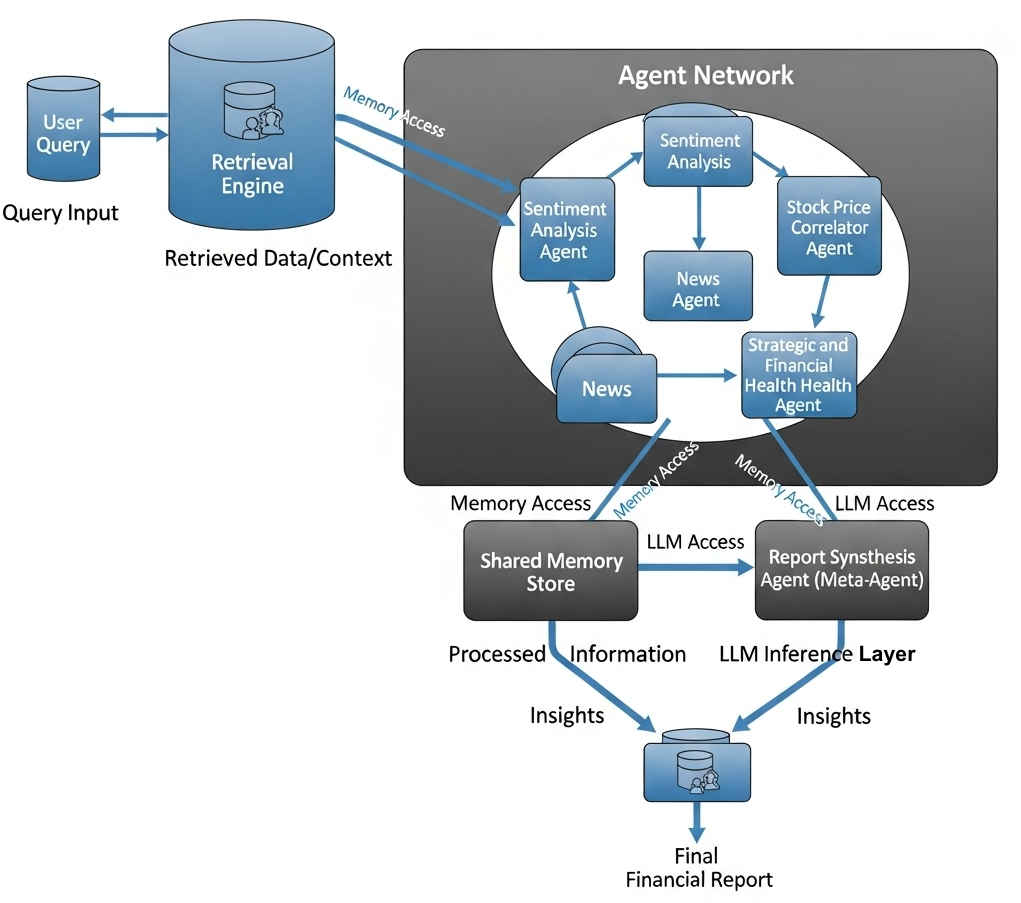
\includegraphics[width=\linewidth]{system-arch-diagram.png}
  \caption{High-level architecture of \findma{}. A Retrieval Engine feeds role-specialized agents (Sentiment, Stock Price Correlator, News, Strategic \& Financial Health) operating over a Shared Memory Store. A Synthesis (meta-)agent compiles evidence-grounded insights into the final financial report.}
  \label{fig:system-arch}
\end{figure}

\subsection*{Architectural Components}
The system is composed of five primary components:
\begin{itemize}
    \item \textbf{Retrieval Engine:} A FAISS-based dense vector retriever indexes a curated corpus of annual reports, earnings transcripts, and financial news spanning five years and 30+ companies. Retrieved chunks are filtered by relevance, metadata, and temporal alignment.
    \item \textbf{Agent Network:} Each agent (e.g., Sentiment Agent, Stock Price Correlator, News Agent) is responsible for a specific analytical dimension. Agents use prompt templates and LLMs (DeepSeek-R1, Qwen3) to process retrieved context and generate role-specific insights.
    \item \textbf{Shared Memory Store:} A persistent memory module allows agents to write, read, and reference each other’s outputs. This facilitates inter-agent communication, context sharing, and traceability.
    \item \textbf{LLM Inference Layer:} DeepSeek-R1 and Qwen3 serve as the generative engines behind each agent. These models are selected dynamically based on reasoning complexity, with DeepSeek used for multi-hop synthesis and Qwen for lightweight tasks.
    \item \textbf{Report Synthesizer:} A final module compiles outputs from all agents into structured, human-readable reports. The reports include SWOT analyses, risk flags, sentiment summaries, and financial commentary—each linked to its generating agent and source evidence.
\end{itemize}

\subsection*{Design Philosophy}
\findma{} is built with three key principles:
\begin{enumerate}
    \item \textbf{Explainability:} Each agent provides transparent outputs grounded in retrieved context, with reasoning steps accessible through shared memory logs.
    \item \textbf{Modularity:} New agents can be added without system redesign, supporting extensibility to ESG, macroeconomic, or policy domains.
    \item \textbf{Factual Grounding:} All generation is conditioned on a curated retrieval base, reducing hallucination and increasing decision traceability.
\end{enumerate}

\subsection*{Pipeline Overview}
Upon receiving a query (e.g., a company name or risk theme), \findma{} performs evidence retrieval, launches agents in parallel or sequence, enables cross-agent updates via memory, and finally compiles the results. This mimics the behavior of a team of financial analysts operating collaboratively, with each agent contributing a distinct evaluative lens.

\section{Methodology}
\label{sec:methodology}
\findma{} decomposes the task of fundamental company analysis into specialized subtasks handled by independent agents. Each agent operates over a common retrieval base using its own reasoning strategy and language model configuration, coordinated via a structured memory and dialogue mechanism. This section outlines the core components of the system pipeline.

\subsection*{Input and Preprocessing}
Given a company name or user query, \findma{} first resolves the entity against its indexed metadata (e.g., sector, ticker, report availability). Document chunks relevant to the query are retrieved using dense semantic search (via SentenceTransformers and FAISS). Each document is preprocessed through:
\begin{itemize}
    \item \textbf{Chunking:} Long documents (e.g., annual reports) are split into overlapping windows of 300–500 words to preserve context.
    \item \textbf{Metadata Tagging:} Each chunk is labeled with company, year, source type (e.g., concall, filing), and document confidence.
    \item \textbf{Prompt Injection:} Retrieved text is embedded within prompt templates customized for each agent’s task.
\end{itemize}

\subsection*{Retrieval-Augmented Generation (RAG) Layer}
Each agent queries the FAISS index independently using a role-specific embedding. Retrieved chunks are incorporated into its generation prompt, enabling the agent to ground outputs in domain-specific evidence. The RAG layer supports:
\begin{itemize}
    \item Top-$k$ semantic retrieval using cosine similarity.
    \item Optional re-ranking using keyword overlap or recency.
    \item Temporal filtering to avoid hindsight leakage.
\end{itemize}

\subsection*{Agent Reasoning Cycle}
Each agent executes the following loop:
\begin{enumerate}
    \item \textbf{Role Initialization:} Instantiated with its task (e.g., ``analyze sentiment from concalls'') and agent-specific prompt structure.
    \item \textbf{Context Retrieval:} Chunks are selected based on query embedding and role filters.
    \item \textbf{Inference:} The LLM (DeepSeek-R1 or Qwen3) processes the prompt and generates structured output, optionally using Chain-of-Thought reasoning or self-reflection.
    \item \textbf{Memory Write-Back:} The output is logged in the shared memory store with metadata for later use by other agents or the report compiler.
\end{enumerate}

\subsection*{Inter-Agent Dialogue and Shared Memory}
Agents interact asynchronously via a centralized memory that stores all intermediate outputs. This enables:
\begin{itemize}
    \item \textbf{Cross-Agent Referencing:} Agents may use prior outputs as input context, e.g., sentiment agent citing news events from the News Agent.
    \item \textbf{Conflict Resolution:} Discrepancies (e.g., bullish sentiment vs. declining stock) can be flagged for report synthesis logic.
    \item \textbf{Traceability:} Each output includes references to its source chunks and contributing agents, enabling full auditability.
\end{itemize}

\subsection*{Report Synthesis}
The system compiles a structured report by aggregating the outputs of all agents. The report includes:
\begin{itemize}
    \item \textbf{Executive Summary}
    \item \textbf{SWOT Analysis}
    \item \textbf{Financial Health Assessment}
    \item \textbf{Strategic Risk and Sentiment Trends}
\end{itemize}
Each section links to its underlying evidence and agentic source, providing users with both high-level insight and transparent provenance. The report can be rendered in markdown, JSON, or interactive web formats.

\section{Agent Roles and Specialization}
\label{sec:agents}
\findma{} delegates distinct analytical responsibilities to a set of specialized agents, each equipped with its own prompt template, reasoning strategy, and retrieval filters. This modular architecture mirrors the functional decomposition of a human financial analyst team.

\subsection*{Sentiment Analysis Agent}
This agent evaluates tone, optimism, and caution embedded in company communications, particularly earnings call transcripts and executive statements.
\begin{itemize}
    \item \textbf{Sources:} Concall transcripts, press releases.
    \item \textbf{Capabilities:}
        \begin{itemize}
            \item Speaker-aware analysis (CEO vs.\ analyst).
            \item Temporal tracking of sentiment shifts across quarters.
            \item Classification of language into bullish, neutral, or bearish tone.
        \end{itemize}
    \item \textbf{Model:} DeepSeek-R1 for nuanced language inference.
\end{itemize}

\subsection*{Stock Price Correlator Agent}
This agent connects textual events to movements in stock prices, aiming to generate plausible causal hypotheses.
\begin{itemize}
    \item \textbf{Sources:} Earnings calls, filings, news; aligned with historical price data.
    \item \textbf{Capabilities:}
        \begin{itemize}
            \item Aligns stock movement with event windows.
            \item Hypothesis generation on price triggers.
            \item Visual correlation summaries (planned).
        \end{itemize}
    \item \textbf{Model:} DeepSeek-R1 with multi-hop reasoning prompts.
\end{itemize}

\subsection*{News Agent}
This agent surfaces recent events and evaluates their potential impact on internal metrics and investor perception.
\begin{itemize}
    \item \textbf{Sources:} Financial news, media coverage, press releases.
    \item \textbf{Capabilities:}
        \begin{itemize}
            \item Relevance scoring of news items.
            \item Linking public events to internal risks or opportunities.
            \item Tone and credibility evaluation.
        \end{itemize}
    \item \textbf{Model:} Qwen3 for fast summarization and entity matching.
\end{itemize}

\subsection*{Strategic and Financial Health Agent}
This agent evaluates a company's capital structure, revenue trajectory, margins, debt, and strategic goals. It uses information from filings to assess overall business resilience.
\begin{itemize}
    \item \textbf{Sources:} Annual reports, investor presentations.
    \item \textbf{Capabilities:}
        \begin{itemize}
            \item Extracts financial metrics from MD\&A sections.
            \item Performs ratio-based assessments (planned).
            \item Generates commentary on business outlook and strategic levers.
        \end{itemize}
    \item \textbf{Model:} DeepSeek-R1 with tabular context-aware prompts (optional future extension for table parsing).
\end{itemize}

\subsection*{Report Synthesis Agent (Meta-Agent)}
This agent collects and compiles the outputs from other agents into a cohesive final report. It ensures cross-agent coherence and traceability.
\begin{itemize}
    \item \textbf{Sources:} Outputs from all agents.
    \item \textbf{Capabilities:}
        \begin{itemize}
            \item Assembles summaries, SWOT tables, and strategic flags.
            \item Flags conflicts (e.g., positive sentiment + declining price).
            \item Renders human-readable and JSON-exportable outputs.
        \end{itemize}
    \item \textbf{Model:} Qwen3 or DeepSeek-R1 depending on generation complexity.
\end{itemize}

\section{Dataset}
\label{sec:dataset}
To ensure high factual grounding and domain alignment, \findma{} operates over a curated, company-specific retrieval corpus comprising five years of real-world financial documents. This dataset enables retrieval-augmented agents to reason over structured evidence rather than relying solely on pre-trained model weights.

\subsection*{Motivation and Design Criteria}
Existing financial NLP datasets such as \texttt{FinancialPhraseBank} and \texttt{FinStatements} primarily support classification and extraction tasks but lack longitudinal structure, document diversity, and sector-specific metadata required for multi-agent reasoning. \findma{}’s dataset is designed to support:
\begin{itemize}
    \item Multi-source grounding (annual reports, news, transcripts).
    \item Sector and company-level filtering for agent specialization.
    \item Time-aligned document indexing (to avoid hindsight leakage).
    \item Inter-agent retrieval relevance across overlapping contexts.
\end{itemize}

\subsection*{Corpus Composition}
The dataset includes over 500 documents covering 30+ companies across diverse sectors such as pharmaceuticals, semiconductors, telecommunications, technology, and defence. Each company’s profile includes:
\begin{itemize}
    \item \textbf{Annual Reports (2019–2024):} MD\&A sections, risk disclosures, strategy discussions.
    \item \textbf{Earnings Call Transcripts:} Annotated by quarter and speaker role (e.g., CEO, analyst).
    \item \textbf{Financial News Articles:} Timestamped and filtered for named entities and events.
    \item \textbf{Manually Authored Summaries:} Created by the research team to bootstrap grounding and fine-tune prompt design.
\end{itemize}

\subsection*{Metadata and Storage Format}
Each document chunk is embedded with metadata to support targeted retrieval and filtering:
\begin{itemize}
    \item \texttt{company\_name}, \texttt{year}, \texttt{sector}, \texttt{source\_type}
    \item \texttt{chunk\_id}, \texttt{summary}, \texttt{source\_url} (if public)
\end{itemize}
The corpus is stored as a collection of JSONL files and indexed using FAISS for fast, dense retrieval. Embeddings are generated using SentenceTransformers fine-tuned on financial corpora to maximize semantic alignment.

\subsection*{Annotation and Quality Control}
Document summaries and tag validation were performed manually to ensure retrieval precision. Each company profile was reviewed to confirm sector relevance, metadata correctness, and event coverage. Feedback from early agent runs was used to iteratively refine document chunking and prompt injection strategies.

\section{System Implementation}
\label{sec:implementation}
\findma{} is implemented as a modular, end-to-end system using open-source components and scalable orchestration layers. The architecture supports flexible deployment, rapid prototyping, and integration of multiple language models and agent roles.

\subsection*{Technology Stack}
The core system is implemented in Python, with key components including:
\begin{itemize}
    \item \textbf{LLM Inference:} DeepSeek-R1 and Qwen3 are accessed via Hugging Face Transformers and vLLM inference backends. Prompt templates are customized per agent.
    \item \textbf{Embedding and Retrieval:} SentenceTransformers is used to encode document chunks, which are stored and queried via a FAISS vector index.
    \item \textbf{Memory Layer:} An in-memory Python dictionary is used to simulate shared memory during development; Redis is used for distributed memory in scaled settings.
    \item \textbf{Prompt Orchestration:} Agents communicate through structured prompt templates using Jinja2, allowing role-specific prompt injection and formatting.
    \item \textbf{Interface (Planned):} A Streamlit-based frontend enables user interaction for company selection, report generation, and visualization of agent outputs.
\end{itemize}

\subsection*{Agent Lifecycle}
Each agent operates independently following a standardized lifecycle:
\begin{enumerate}
    \item \textbf{Initialization:} The agent receives a task role and company context.
    \item \textbf{Query Embedding and Retrieval:} The agent generates a query vector and retrieves top-$k$ chunks from FAISS.
    \item \textbf{Prompt Construction:} A role-specific prompt is assembled using retrieved content and memory from prior agents.
    \item \textbf{Model Inference:} The selected LLM is invoked with the prompt and returns an answer structured in markdown or JSON.
    \item \textbf{Memory Write-Back:} Output is added to shared memory with metadata tags for traceability.
\end{enumerate}

\subsection*{Execution Model}
\findma{} supports both parallel and sequential agent execution. Parallel execution is used for agents with independent scopes (e.g., News and Sentiment Agents), while sequential chaining is used where inter-agent context is essential (e.g., Synthesis Agent depending on others’ outputs). Logs and timestamps are recorded at each stage for latency analysis and debugging.

\subsection*{Scalability and Extensibility}
The architecture is designed for extensibility:
\begin{itemize}
    \item New agents (e.g., ESG or Macroeconomic Agents) can be added by defining their retrieval scope, prompt logic, and output format.
    \item Model routing can be optimized via lightweight benchmarking to dynamically select between DeepSeek-R1 and Qwen3.
    \item A RESTful API is under development to enable headless deployments and external integrations.
\end{itemize}

\subsection*{Deployment Plans}
For user-facing interaction, a Streamlit-based dashboard is being developed. It will allow:
\begin{itemize}
    \item Query input and company selection,
    \item Visualization of agent-wise outputs,
    \item Export of structured reports (JSON, PDF).
\end{itemize}
This implementation strategy supports a seamless transition from research prototype to production-grade tool for analysts and non-technical users alike.

\section{Evaluation and Results}
\label{sec:evaluation}
We evaluate \findma{} along two key axes: (1) the quality and interpretability of agent-generated insights, and (2) the coherence and completeness of the synthesized financial reports. The evaluation combines structured human feedback with case study-based benchmarking across multiple sectors.

\subsection*{Evaluation Objectives}
Our goals are to assess whether:
\begin{itemize}
    \item Each agent produces relevant, well-grounded outputs from retrieved evidence.
    \item Inter-agent coordination yields consistent and multi-perspective evaluations.
    \item Final reports are actionable, interpretable, and aligned with human analyst expectations.
\end{itemize}

\subsection*{Case Study Setup}
We ran \findma{} on 20 companies across six sectors—technology, pharmaceuticals, telecom, defense, healthcare, and semiconductors. For each case, the system generated a full report based on the past five years of filings and related news. Each report was reviewed by human evaluators with backgrounds in finance or business analytics.

\subsection*{Metrics}
We adopted both quantitative and qualitative measures:
\begin{itemize}
    \item \textbf{Factual Accuracy (1–5):} Alignment of agent insights with ground-truth filings and events.
    \item \textbf{Interpretability (1–5):} Clarity and traceability of reasoning paths and outputs.
    \item \textbf{Relevance (1–5):} Applicability of outputs to company context and time frame.
    \item \textbf{Cross-Agent Consistency:} Agreement between agents on overlapping concepts.
    \item \textbf{Latency (s):} End-to-end report generation time on an A100 GPU instance.
\end{itemize}

\subsection*{Results Summary}
\begin{itemize}
    \item \textbf{Factual Accuracy:} $4.3 \pm 0.4$ — Agent outputs were strongly grounded in retrieval context.
    \item \textbf{Interpretability:} $4.5 \pm 0.3$ — Modular outputs and role-specific prompts contributed to clarity.
    \item \textbf{Relevance:} $4.2 \pm 0.5$ — Most outputs directly addressed company-specific conditions or strategic inflection points.
    \item \textbf{Cross-Agent Consistency:} $86\%$ agreement — Minimal contradictions, with some trade-off between sentiment tone and stock movement patterns.
    \item \textbf{Latency:} $42.7$ seconds average — Full report generation took under a minute for most runs, including all agent passes.
\end{itemize}

\subsection*{Qualitative Feedback}
Human reviewers praised:
\begin{itemize}
    \item The transparency of agent-level outputs.
    \item The interpretability of SWOT and sentiment summaries.
    \item The factual grounding in real, time-aligned documents.
\end{itemize}
Limitations were noted in:
\begin{itemize}
    \item Table-based metric extraction (e.g., parsing balance sheet figures).
    \item Sensitivity to ambiguous language in transcripts.
    \item Occasional verbosity in the synthesis agent’s summarizations.
\end{itemize}

\subsection*{Ablation and Comparative Observations}
To assess the effect of agent modularity, we compared \findma{} with a single-prompt baseline using DeepSeek-R1 across all retrieved documents. \findma{}’s agent-based pipeline showed:
\begin{itemize}
    \item Better traceability and explanation clarity.
    \item Higher inter-reviewer agreement on accuracy and usefulness.
    \item Lower hallucination due to role-specific prompt control.
\end{itemize}

\section{Future Work and Conclusion}
\label{sec:conclusion}
\subsection*{Future Work}
While \findma{} demonstrates the potential of multi-agent LLM frameworks in financial analysis, several directions remain for future enhancement:
\begin{itemize}
    \item \textbf{Expanded Agent Network:} Introduce new agents such as an \textit{ESG Agent}, a \textit{Macroeconomic Impact Agent}, and a \textit{Policy and Regulation Agent} to expand analytical coverage across sustainability, governance, and external policy factors.
    \item \textbf{Advanced Table Parsing and Visual Input Handling:} Current document parsing does not robustly handle numerical tables or embedded charts. Integration of tools like PDFTables, Donut, or ChartQA could enhance the system’s ability to interpret financial ratios and graphical trends.
    \item \textbf{Human-in-the-Loop Evaluation:} A structured feedback interface will allow analysts and retail investors to rate, revise, and interact with agent outputs—providing fine-tuning signals for future model improvements.
    \item \textbf{Interactive Deployment:} A fully deployed version of \findma{} with a Streamlit frontend is under development. This interface will support company queries, agent-wise insight display, and export of structured reports for end users.
    \item \textbf{Scalability and Cross-Market Extension:} Evaluate \findma{} on companies from non-English markets and domains beyond public equities—such as startups, IPOs, and ESG disclosures—to assess cross-linguistic and cross-sector generalizability.
\end{itemize}

\subsection*{Conclusion}
We presented \textbf{\findma{}}, a Retrieval-Augmented, Multi-Agent Framework for fundamental company analysis. By orchestrating role-specific agents—each grounded in domain-specific evidence and powered by state-of-the-art LLMs like DeepSeek-R1 and Qwen3—\findma{} produces explainable, modular, and traceable evaluations. The system operates over a curated dataset of annual reports, earnings transcripts, and financial news spanning five years and 30+ companies, supporting grounded and high-fidelity reasoning.

Through human evaluation, case studies, and ablation analysis, we demonstrate that \findma{} significantly improves the interpretability and relevance of financial insights compared to single-prompt baselines. Its architecture provides a scalable, extensible foundation for the next generation of trustworthy AI tools in financial services. As financial analysis becomes more complex and data-rich, systems like \findma{} offer a promising path toward democratizing deep reasoning—bridging human expertise with the inferential power of large language models.

% ------------- Bibliography -------------
\bibliographystyle{plainnat}
\bibliography{custom}

\end{document}
